% !TEX root = main.tex

\begin{figure}
    \centering
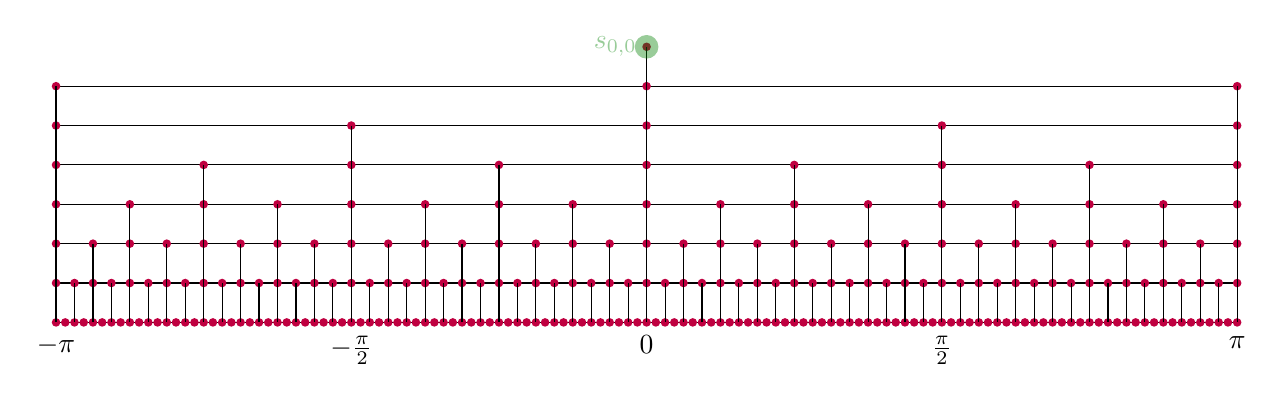
\begin{tikzpicture}[scale=0.5]

  \pgfmathsetmacro{\xlimit}{30}
  \pgfmathsetmacro{\ylimit}{7}

  \foreach \yunscaled in {0,..., \ylimit} 
  {
    \pgfmathsetmacro{\y}{\yunscaled}
    \pgfmathsetmacro{\lognumpoints}{\ylimit-\y}
    \pgfmathsetmacro{\numpoints}{2^\lognumpoints}
    \pgfmathsetmacro{\z}{\xlimit/\numpoints}
    \ifnum\y=\ylimit{
      % Do nothing
    }
    \else{
      \draw (0,\y) -- (\xlimit,\y);
      \foreach \i in {0,...,\numpoints}{
        \pgfmathsetmacro{\x}{\z * \i}
        \draw (\x,\y) node[circle,fill,inner sep=1.1pt, color=purple]{}; % Marked point
      \draw (\x,\y) -- (\x,0); % Vertical line
      }
    }
    \fi
  }
  \draw (\xlimit/2,\ylimit) node[circle,fill,inner sep=1.1pt, color=purple]{}; % Marked point
  \draw (\xlimit/2,\ylimit) -- (\xlimit/2,0); % Vertical line


  % Label horizontal lines
  \draw (0,-0.1) node[below] {$-\pi$};
  \draw (\xlimit/4,-0.1) node[below] {$-\frac \pi 2$};
  \draw (\xlimit/2,-0.1) node[below] {$0$};
  \draw (\xlimit*3/4,-0.1) node[below] {$\frac \pi 2$};
  \draw (\xlimit,-0.1) node[below] {$\pi$};

\definecolor{mygreen}{RGB}{0, 128, 0}

\fill [mygreen, opacity=0.4] (\xlimit/2, 7) circle (0.3)
node[left] {$s_{0,0}$};

  % \tikzmath{
  %   \curx = 0;
  %   for \step in {1,...,2}{
  %     {\draw [magenta,-, double=magenta, double distance=4\pgflinewidth, opacity=0.4] (\curx, \ylimit-\step) -- (\curx, \ylimit-\step-1);};
  % };}
  
\end{tikzpicture}
\captionof{figure}{A convenient representation of the dyadic grid in the Böttcher coordinates.
 The horizontal axis is the external angle $\mathrm{Arg}(\psi^{-1}(z))$, and the vertical axis is the equipotential $|\psi ^{-1}(z)|$, plotted on a log scale. 
 The rightmost edge is glued to the leftmost edge.
 Stations are marked in red, and the segments connecting adjacent stations are tracks. An express track is a vertical segment, 
 while a peripheral track is a horizontal segment.
 The central station is highlighted in green. The bottom row represents the Julia set $\mathcal J$.
  }  \label{fig:dyadic_grid}
\end{figure} 
